\documentclass[]{article}
\usepackage{lmodern}
\usepackage{amssymb,amsmath}
\usepackage{ifxetex,ifluatex}
\usepackage{fixltx2e} % provides \textsubscript
\ifnum 0\ifxetex 1\fi\ifluatex 1\fi=0 % if pdftex
  \usepackage[T1]{fontenc}
  \usepackage[utf8]{inputenc}
\else % if luatex or xelatex
  \ifxetex
    \usepackage{mathspec}
  \else
    \usepackage{fontspec}
  \fi
  \defaultfontfeatures{Ligatures=TeX,Scale=MatchLowercase}
\fi
% use upquote if available, for straight quotes in verbatim environments
\IfFileExists{upquote.sty}{\usepackage{upquote}}{}
% use microtype if available
\IfFileExists{microtype.sty}{%
\usepackage{microtype}
\UseMicrotypeSet[protrusion]{basicmath} % disable protrusion for tt fonts
}{}
\usepackage[margin=1in]{geometry}
\usepackage{hyperref}
\hypersetup{unicode=true,
            pdfborder={0 0 0},
            breaklinks=true}
\urlstyle{same}  % don't use monospace font for urls
\usepackage{color}
\usepackage{fancyvrb}
\newcommand{\VerbBar}{|}
\newcommand{\VERB}{\Verb[commandchars=\\\{\}]}
\DefineVerbatimEnvironment{Highlighting}{Verbatim}{commandchars=\\\{\}}
% Add ',fontsize=\small' for more characters per line
\usepackage{framed}
\definecolor{shadecolor}{RGB}{248,248,248}
\newenvironment{Shaded}{\begin{snugshade}}{\end{snugshade}}
\newcommand{\KeywordTok}[1]{\textcolor[rgb]{0.13,0.29,0.53}{\textbf{#1}}}
\newcommand{\DataTypeTok}[1]{\textcolor[rgb]{0.13,0.29,0.53}{#1}}
\newcommand{\DecValTok}[1]{\textcolor[rgb]{0.00,0.00,0.81}{#1}}
\newcommand{\BaseNTok}[1]{\textcolor[rgb]{0.00,0.00,0.81}{#1}}
\newcommand{\FloatTok}[1]{\textcolor[rgb]{0.00,0.00,0.81}{#1}}
\newcommand{\ConstantTok}[1]{\textcolor[rgb]{0.00,0.00,0.00}{#1}}
\newcommand{\CharTok}[1]{\textcolor[rgb]{0.31,0.60,0.02}{#1}}
\newcommand{\SpecialCharTok}[1]{\textcolor[rgb]{0.00,0.00,0.00}{#1}}
\newcommand{\StringTok}[1]{\textcolor[rgb]{0.31,0.60,0.02}{#1}}
\newcommand{\VerbatimStringTok}[1]{\textcolor[rgb]{0.31,0.60,0.02}{#1}}
\newcommand{\SpecialStringTok}[1]{\textcolor[rgb]{0.31,0.60,0.02}{#1}}
\newcommand{\ImportTok}[1]{#1}
\newcommand{\CommentTok}[1]{\textcolor[rgb]{0.56,0.35,0.01}{\textit{#1}}}
\newcommand{\DocumentationTok}[1]{\textcolor[rgb]{0.56,0.35,0.01}{\textbf{\textit{#1}}}}
\newcommand{\AnnotationTok}[1]{\textcolor[rgb]{0.56,0.35,0.01}{\textbf{\textit{#1}}}}
\newcommand{\CommentVarTok}[1]{\textcolor[rgb]{0.56,0.35,0.01}{\textbf{\textit{#1}}}}
\newcommand{\OtherTok}[1]{\textcolor[rgb]{0.56,0.35,0.01}{#1}}
\newcommand{\FunctionTok}[1]{\textcolor[rgb]{0.00,0.00,0.00}{#1}}
\newcommand{\VariableTok}[1]{\textcolor[rgb]{0.00,0.00,0.00}{#1}}
\newcommand{\ControlFlowTok}[1]{\textcolor[rgb]{0.13,0.29,0.53}{\textbf{#1}}}
\newcommand{\OperatorTok}[1]{\textcolor[rgb]{0.81,0.36,0.00}{\textbf{#1}}}
\newcommand{\BuiltInTok}[1]{#1}
\newcommand{\ExtensionTok}[1]{#1}
\newcommand{\PreprocessorTok}[1]{\textcolor[rgb]{0.56,0.35,0.01}{\textit{#1}}}
\newcommand{\AttributeTok}[1]{\textcolor[rgb]{0.77,0.63,0.00}{#1}}
\newcommand{\RegionMarkerTok}[1]{#1}
\newcommand{\InformationTok}[1]{\textcolor[rgb]{0.56,0.35,0.01}{\textbf{\textit{#1}}}}
\newcommand{\WarningTok}[1]{\textcolor[rgb]{0.56,0.35,0.01}{\textbf{\textit{#1}}}}
\newcommand{\AlertTok}[1]{\textcolor[rgb]{0.94,0.16,0.16}{#1}}
\newcommand{\ErrorTok}[1]{\textcolor[rgb]{0.64,0.00,0.00}{\textbf{#1}}}
\newcommand{\NormalTok}[1]{#1}
\usepackage{graphicx,grffile}
\makeatletter
\def\maxwidth{\ifdim\Gin@nat@width>\linewidth\linewidth\else\Gin@nat@width\fi}
\def\maxheight{\ifdim\Gin@nat@height>\textheight\textheight\else\Gin@nat@height\fi}
\makeatother
% Scale images if necessary, so that they will not overflow the page
% margins by default, and it is still possible to overwrite the defaults
% using explicit options in \includegraphics[width, height, ...]{}
\setkeys{Gin}{width=\maxwidth,height=\maxheight,keepaspectratio}
\IfFileExists{parskip.sty}{%
\usepackage{parskip}
}{% else
\setlength{\parindent}{0pt}
\setlength{\parskip}{6pt plus 2pt minus 1pt}
}
\setlength{\emergencystretch}{3em}  % prevent overfull lines
\providecommand{\tightlist}{%
  \setlength{\itemsep}{0pt}\setlength{\parskip}{0pt}}
\setcounter{secnumdepth}{0}
% Redefines (sub)paragraphs to behave more like sections
\ifx\paragraph\undefined\else
\let\oldparagraph\paragraph
\renewcommand{\paragraph}[1]{\oldparagraph{#1}\mbox{}}
\fi
\ifx\subparagraph\undefined\else
\let\oldsubparagraph\subparagraph
\renewcommand{\subparagraph}[1]{\oldsubparagraph{#1}\mbox{}}
\fi

%%% Use protect on footnotes to avoid problems with footnotes in titles
\let\rmarkdownfootnote\footnote%
\def\footnote{\protect\rmarkdownfootnote}

%%% Change title format to be more compact
\usepackage{titling}

% Create subtitle command for use in maketitle
\newcommand{\subtitle}[1]{
  \posttitle{
    \begin{center}\large#1\end{center}
    }
}

\setlength{\droptitle}{-2em}

  \title{}
    \pretitle{\vspace{\droptitle}}
  \posttitle{}
    \author{}
    \preauthor{}\postauthor{}
    \date{}
    \predate{}\postdate{}
  

\begin{document}

\begin{Shaded}
\begin{Highlighting}[]
\NormalTok{knitr}\OperatorTok{::}\NormalTok{opts_chunk}\OperatorTok{$}\KeywordTok{set}\NormalTok{(}\DataTypeTok{echo =} \OtherTok{TRUE}\NormalTok{)}
\NormalTok{nsims <-}\StringTok{ }\DecValTok{100000} \CommentTok{#set number of simulations}
\KeywordTok{library}\NormalTok{(mvtnorm)}
\KeywordTok{library}\NormalTok{(afex)}
\KeywordTok{library}\NormalTok{(emmeans)}
\KeywordTok{library}\NormalTok{(ggplot2)}
\KeywordTok{library}\NormalTok{(gridExtra)}
\KeywordTok{library}\NormalTok{(reshape2)}
\KeywordTok{library}\NormalTok{(pwr)}

\CommentTok{# Install functions from GitHub by running the code below:}
\KeywordTok{source}\NormalTok{(}\StringTok{"https://raw.githubusercontent.com/Lakens/ANOVA_power_simulation/master/ANOVA_design.R"}\NormalTok{)}
\KeywordTok{source}\NormalTok{(}\StringTok{"https://raw.githubusercontent.com/Lakens/ANOVA_power_simulation/master/ANOVA_power.R"}\NormalTok{)}
\end{Highlighting}
\end{Shaded}

\subsection{Analytic power functions}\label{analytic-power-functions}

For some designs it is possible to calculate power analytically, using
closed functions.

\section{2x2 Between Subject
Interaction}\label{x2-between-subject-interaction}

\begin{Shaded}
\begin{Highlighting}[]
\NormalTok{string <-}\StringTok{ "2b*2b"}
\NormalTok{n <-}\StringTok{ }\DecValTok{20}
\NormalTok{mu <-}\StringTok{ }\KeywordTok{c}\NormalTok{(}\DecValTok{20}\NormalTok{, }\DecValTok{20}\NormalTok{, }\DecValTok{20}\NormalTok{, }\DecValTok{25}\NormalTok{) }\CommentTok{#All means are equal - so there is no real difference.}
\CommentTok{# Enter means in the order that matches the labels below.}
\NormalTok{sd <-}\StringTok{ }\DecValTok{5}
\NormalTok{r <-}\StringTok{ }\DecValTok{0} 
\CommentTok{# (note that since we simulate a between design, the correlation between variables }
\CommentTok{# will be 0, regardless of what you enter here, but the value must be set).}
\NormalTok{p_adjust =}\StringTok{ "none"}
\CommentTok{# "none" means we do not correct for multiple comparisons}
\NormalTok{labelnames <-}\StringTok{ }\KeywordTok{c}\NormalTok{(}\StringTok{"Factor_A"}\NormalTok{, }\StringTok{"a1"}\NormalTok{, }\StringTok{"a2"}\NormalTok{, }\StringTok{"Factor_B"}\NormalTok{, }\StringTok{"b1"}\NormalTok{, }\StringTok{"b2"}\NormalTok{) }\CommentTok{#}
\CommentTok{# the label names should be in the order of the means specified above.}

\NormalTok{design_result <-}\StringTok{ }\KeywordTok{ANOVA_design}\NormalTok{(}\DataTypeTok{string =}\NormalTok{ string,}
                   \DataTypeTok{n =}\NormalTok{ n, }
                   \DataTypeTok{mu =}\NormalTok{ mu, }
                   \DataTypeTok{sd =}\NormalTok{ sd, }
                   \DataTypeTok{r =}\NormalTok{ r, }
                   \DataTypeTok{p_adjust =}\NormalTok{ p_adjust,}
                   \DataTypeTok{labelnames =}\NormalTok{ labelnames)}
\end{Highlighting}
\end{Shaded}

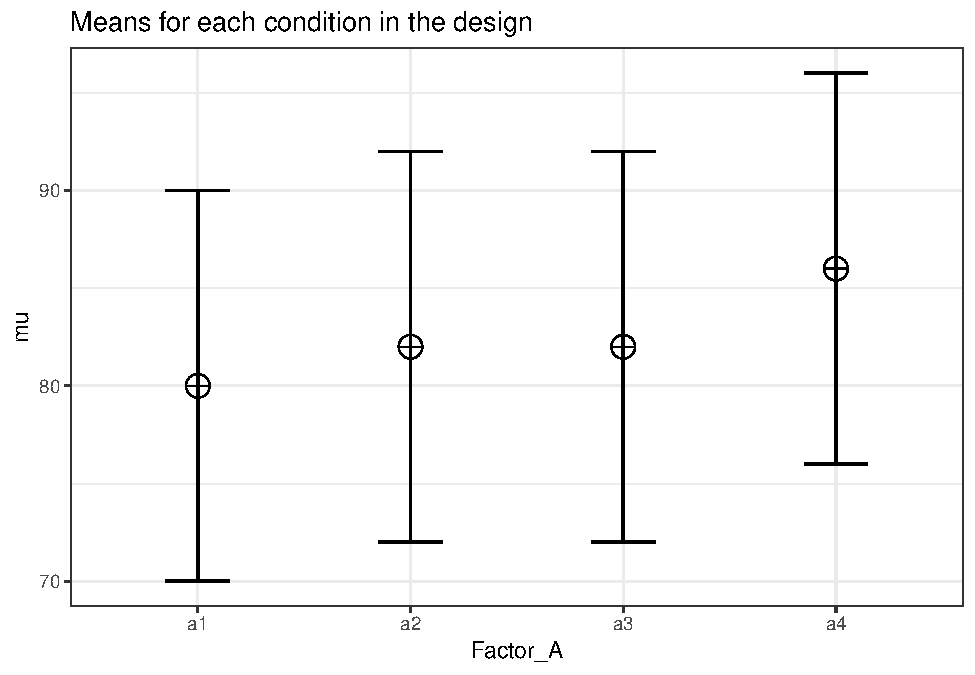
\includegraphics{4.3_analytic_power_functions_files/figure-latex/unnamed-chunk-1-1.pdf}

\begin{Shaded}
\begin{Highlighting}[]
\NormalTok{alpha_level <-}\StringTok{ }\FloatTok{0.05} \CommentTok{#We set the alpha level at 0.05. }

\NormalTok{power_result <-}\StringTok{ }\KeywordTok{ANOVA_power}\NormalTok{(design_result, }\DataTypeTok{alpha_level =}\NormalTok{ alpha_level, }\DataTypeTok{nsims =}\NormalTok{ nsims)}
\end{Highlighting}
\end{Shaded}

\begin{verbatim}
## Power and Effect sizes for ANOVA tests
##                          power effect size
## anova_Factor_A          59.738      0.0622
## anova_Factor_B          59.851      0.0623
## anova_Factor_A:Factor_B 59.837      0.0622
## 
## Power and Effect sizes for contrasts
##                                                    power effect size
## p_Factor_A_a1_Factor_B_b1_Factor_A_a1_Factor_B_b2  4.956     -0.0002
## p_Factor_A_a1_Factor_B_b1_Factor_A_a2_Factor_B_b1  5.039     -0.0008
## p_Factor_A_a1_Factor_B_b1_Factor_A_a2_Factor_B_b2 86.889      1.0201
## p_Factor_A_a1_Factor_B_b2_Factor_A_a2_Factor_B_b1  4.898     -0.0006
## p_Factor_A_a1_Factor_B_b2_Factor_A_a2_Factor_B_b2 86.925      1.0200
## p_Factor_A_a2_Factor_B_b1_Factor_A_a2_Factor_B_b2 86.724      1.0208
\end{verbatim}

Mathematically the interaction effect is computed as the difference
between a cell mean and the grand mean, the marginal mean in row i and
the grand mean, and the marginal mean in column j and grand mean. For
example, for the very hungry-banana condition this is 25 (the value in
the cell) - (21.25 {[}the grand mean{]} + 1.25 {[}the marginal mean in
row 2, 22.5, minus the grand mean of 21.25{]} + 1.25 {[}the marginal
mean in column 2, 22.5, minus the grand mean of 21.25{]}). 25 - (21.25 +
(22.5-21.25) + (22.5-21.25)) = 1.25.

We can repeat this for every cell, and get for no hunger-apple: 20 -
(21.25 + (20-21.25) + (20-21.25)) = 1.25, for very hungry apple: 20 -
(21.25 + (22.5-21.25) + (20-21.25)) = 1.25, and no hunger-banana: 20 -
(21.25 + (20-21.25) + (22.5-21.25)) = 1.25. These values are used to
calculate the sum of squares.

\begin{Shaded}
\begin{Highlighting}[]
\NormalTok{mean_mat <-}\StringTok{ }\KeywordTok{t}\NormalTok{(}\KeywordTok{matrix}\NormalTok{(mu, }
                     \DataTypeTok{nrow =} \DecValTok{2}\NormalTok{,}
                     \DataTypeTok{ncol =} \DecValTok{2}\NormalTok{)) }\CommentTok{#Create a mean matrix}
\KeywordTok{rownames}\NormalTok{(mean_mat) <-}\StringTok{ }\KeywordTok{c}\NormalTok{(}\StringTok{"a1"}\NormalTok{, }\StringTok{"a2"}\NormalTok{)}
\KeywordTok{colnames}\NormalTok{(mean_mat) <-}\StringTok{ }\KeywordTok{c}\NormalTok{(}\StringTok{"b1"}\NormalTok{, }\StringTok{"b2"}\NormalTok{)}
\NormalTok{mean_mat}
\end{Highlighting}
\end{Shaded}

\begin{verbatim}
##    b1 b2
## a1 20 20
## a2 20 25
\end{verbatim}

\begin{Shaded}
\begin{Highlighting}[]
\NormalTok{a1 <-}\StringTok{ }\NormalTok{mean_mat[}\DecValTok{1}\NormalTok{,}\DecValTok{1}\NormalTok{] }\OperatorTok{-}\StringTok{ }\NormalTok{(}\KeywordTok{mean}\NormalTok{(mean_mat) }\OperatorTok{+}\StringTok{ }\NormalTok{(}\KeywordTok{mean}\NormalTok{(mean_mat[}\DecValTok{1}\NormalTok{,]) }\OperatorTok{-}\StringTok{ }\KeywordTok{mean}\NormalTok{(mean_mat)) }\OperatorTok{+}\StringTok{ }\NormalTok{(}\KeywordTok{mean}\NormalTok{(mean_mat[,}\DecValTok{1}\NormalTok{]) }\OperatorTok{-}\StringTok{ }\KeywordTok{mean}\NormalTok{(mean_mat)))}
\NormalTok{a2 <-}\StringTok{ }\NormalTok{mean_mat[}\DecValTok{1}\NormalTok{,}\DecValTok{2}\NormalTok{] }\OperatorTok{-}\StringTok{ }\NormalTok{(}\KeywordTok{mean}\NormalTok{(mean_mat) }\OperatorTok{+}\StringTok{ }\NormalTok{(}\KeywordTok{mean}\NormalTok{(mean_mat[}\DecValTok{1}\NormalTok{,]) }\OperatorTok{-}\StringTok{ }\KeywordTok{mean}\NormalTok{(mean_mat)) }\OperatorTok{+}\StringTok{ }\NormalTok{(}\KeywordTok{mean}\NormalTok{(mean_mat[,}\DecValTok{2}\NormalTok{]) }\OperatorTok{-}\StringTok{ }\KeywordTok{mean}\NormalTok{(mean_mat)))}
\NormalTok{b1 <-}\StringTok{ }\NormalTok{mean_mat[}\DecValTok{2}\NormalTok{,}\DecValTok{1}\NormalTok{] }\OperatorTok{-}\StringTok{ }\NormalTok{(}\KeywordTok{mean}\NormalTok{(mean_mat) }\OperatorTok{+}\StringTok{ }\NormalTok{(}\KeywordTok{mean}\NormalTok{(mean_mat[}\DecValTok{2}\NormalTok{,]) }\OperatorTok{-}\StringTok{ }\KeywordTok{mean}\NormalTok{(mean_mat)) }\OperatorTok{+}\StringTok{ }\NormalTok{(}\KeywordTok{mean}\NormalTok{(mean_mat[,}\DecValTok{1}\NormalTok{]) }\OperatorTok{-}\StringTok{ }\KeywordTok{mean}\NormalTok{(mean_mat)))}
\NormalTok{b2 <-}\StringTok{ }\NormalTok{mean_mat[}\DecValTok{2}\NormalTok{,}\DecValTok{2}\NormalTok{] }\OperatorTok{-}\StringTok{ }\NormalTok{(}\KeywordTok{mean}\NormalTok{(mean_mat) }\OperatorTok{+}\StringTok{ }\NormalTok{(}\KeywordTok{mean}\NormalTok{(mean_mat[}\DecValTok{2}\NormalTok{,]) }\OperatorTok{-}\StringTok{ }\KeywordTok{mean}\NormalTok{(mean_mat)) }\OperatorTok{+}\StringTok{ }\NormalTok{(}\KeywordTok{mean}\NormalTok{(mean_mat[,}\DecValTok{2}\NormalTok{]) }\OperatorTok{-}\StringTok{ }\KeywordTok{mean}\NormalTok{(mean_mat)))}
\KeywordTok{c}\NormalTok{(a1, a2, b1, b2)}
\end{Highlighting}
\end{Shaded}

\begin{verbatim}
## [1]  1.25 -1.25 -1.25  1.25
\end{verbatim}

\begin{Shaded}
\begin{Highlighting}[]
\NormalTok{SS_ab <-}\StringTok{ }\NormalTok{n }\OperatorTok{*}\StringTok{ }\KeywordTok{sum}\NormalTok{(}\KeywordTok{c}\NormalTok{(a1, a2, b1, b2)}\OperatorTok{^}\DecValTok{2}\NormalTok{)}
\end{Highlighting}
\end{Shaded}

The sum of squares is dependent on the sample size. The larger the
sample size, the larger the sum of squares, and therefore (all else
equal) the larger the \emph{F}-statistic, and the smaller the
\emph{p}-value. We see from the simulations that all three tests have
the same effect size, and therefore the same power.

We calculate Cohen's f following the \[f = \frac{\sigma_m}{\sigma}\].
The calculation of \(\sigma_m\) depends on the design. For a 2x2
interaction it is based on the additive effect, or the residuals after
removing main effects of factor A and B.

\begin{Shaded}
\begin{Highlighting}[]
\CommentTok{#We calculate Cohen's f following the f$\textbackslash{}sigma_m}
\NormalTok{f <-}\StringTok{ }\KeywordTok{sqrt}\NormalTok{(}\KeywordTok{sum}\NormalTok{(}\KeywordTok{c}\NormalTok{(a1, a2, b1, b2)}\OperatorTok{^}\DecValTok{2}\NormalTok{)}\OperatorTok{/}\KeywordTok{length}\NormalTok{(mu))}\OperatorTok{/}\NormalTok{sd }\CommentTok{#based on G*power manual page 28}

\CommentTok{#Analytic power formula for interaction}
\NormalTok{k1 <-}\StringTok{ }\DecValTok{2} \CommentTok{#levels in factor 1}
\NormalTok{k2 <-}\StringTok{ }\DecValTok{2} \CommentTok{#levels in factor 1}
\NormalTok{m <-}\StringTok{ }\DecValTok{1} \CommentTok{#number of measurement per group (1 because between design)}
\NormalTok{e <-}\StringTok{ }\DecValTok{1} \CommentTok{#non-spericity correction}
\NormalTok{r <-}\StringTok{ }\FloatTok{0.0} \CommentTok{#correlation between dependent variables (0 in a between design)}
\NormalTok{alpha <-}\StringTok{ }\FloatTok{0.05} \CommentTok{#alpha level for each test}
\NormalTok{df1 <-}\StringTok{ }\NormalTok{(k1}\DecValTok{-1}\NormalTok{) }\OperatorTok{*}\StringTok{ }\NormalTok{(k2}\DecValTok{-1}\NormalTok{) }\OperatorTok{*}\StringTok{ }\NormalTok{e }\CommentTok{#df for effect in interaction}
\NormalTok{df2 <-}\StringTok{ }\NormalTok{(n }\OperatorTok{*}\StringTok{ }\NormalTok{(k1}\OperatorTok{*}\NormalTok{k2) }\OperatorTok{-}\StringTok{ }\NormalTok{(k1}\OperatorTok{*}\NormalTok{k2)) }\OperatorTok{*}\StringTok{ }\NormalTok{e }\CommentTok{#df_error}
\NormalTok{lambda <-}\StringTok{ }\NormalTok{(k1}\OperatorTok{*}\NormalTok{k2) }\OperatorTok{*}\StringTok{ }\NormalTok{n }\OperatorTok{*}\StringTok{ }\NormalTok{(m}\OperatorTok{/}\NormalTok{(}\DecValTok{1} \OperatorTok{+}\StringTok{ }\NormalTok{(m }\OperatorTok{-}\StringTok{ }\DecValTok{1}\NormalTok{) }\OperatorTok{*}\StringTok{ }\NormalTok{r)) }\OperatorTok{*}\StringTok{ }\NormalTok{f}\OperatorTok{^}\DecValTok{2} \CommentTok{# lambda}
\NormalTok{F_critical <-}\StringTok{ }\KeywordTok{qf}\NormalTok{(alpha, df1, df2, }\DataTypeTok{lower.tail=}\OtherTok{FALSE}\NormalTok{) }\CommentTok{# Critical F-Value}
\NormalTok{pow <-}\StringTok{ }\KeywordTok{pf}\NormalTok{(F_critical, df1, df2, lambda, }\DataTypeTok{lower.tail =} \OtherTok{FALSE}\NormalTok{) }\CommentTok{# power}
\NormalTok{pow }\CommentTok{#power}
\end{Highlighting}
\end{Shaded}

\begin{verbatim}
## [1] 0.5978655
\end{verbatim}

\subsection{Two by two ANOVA, within
design}\label{two-by-two-anova-within-design}

Potvin \& Schutz (2000) simulate a wide range of repeated measure
designs. The give an example of a 3x3 design, with the following
correlation matrix:

\begin{figure}
\centering
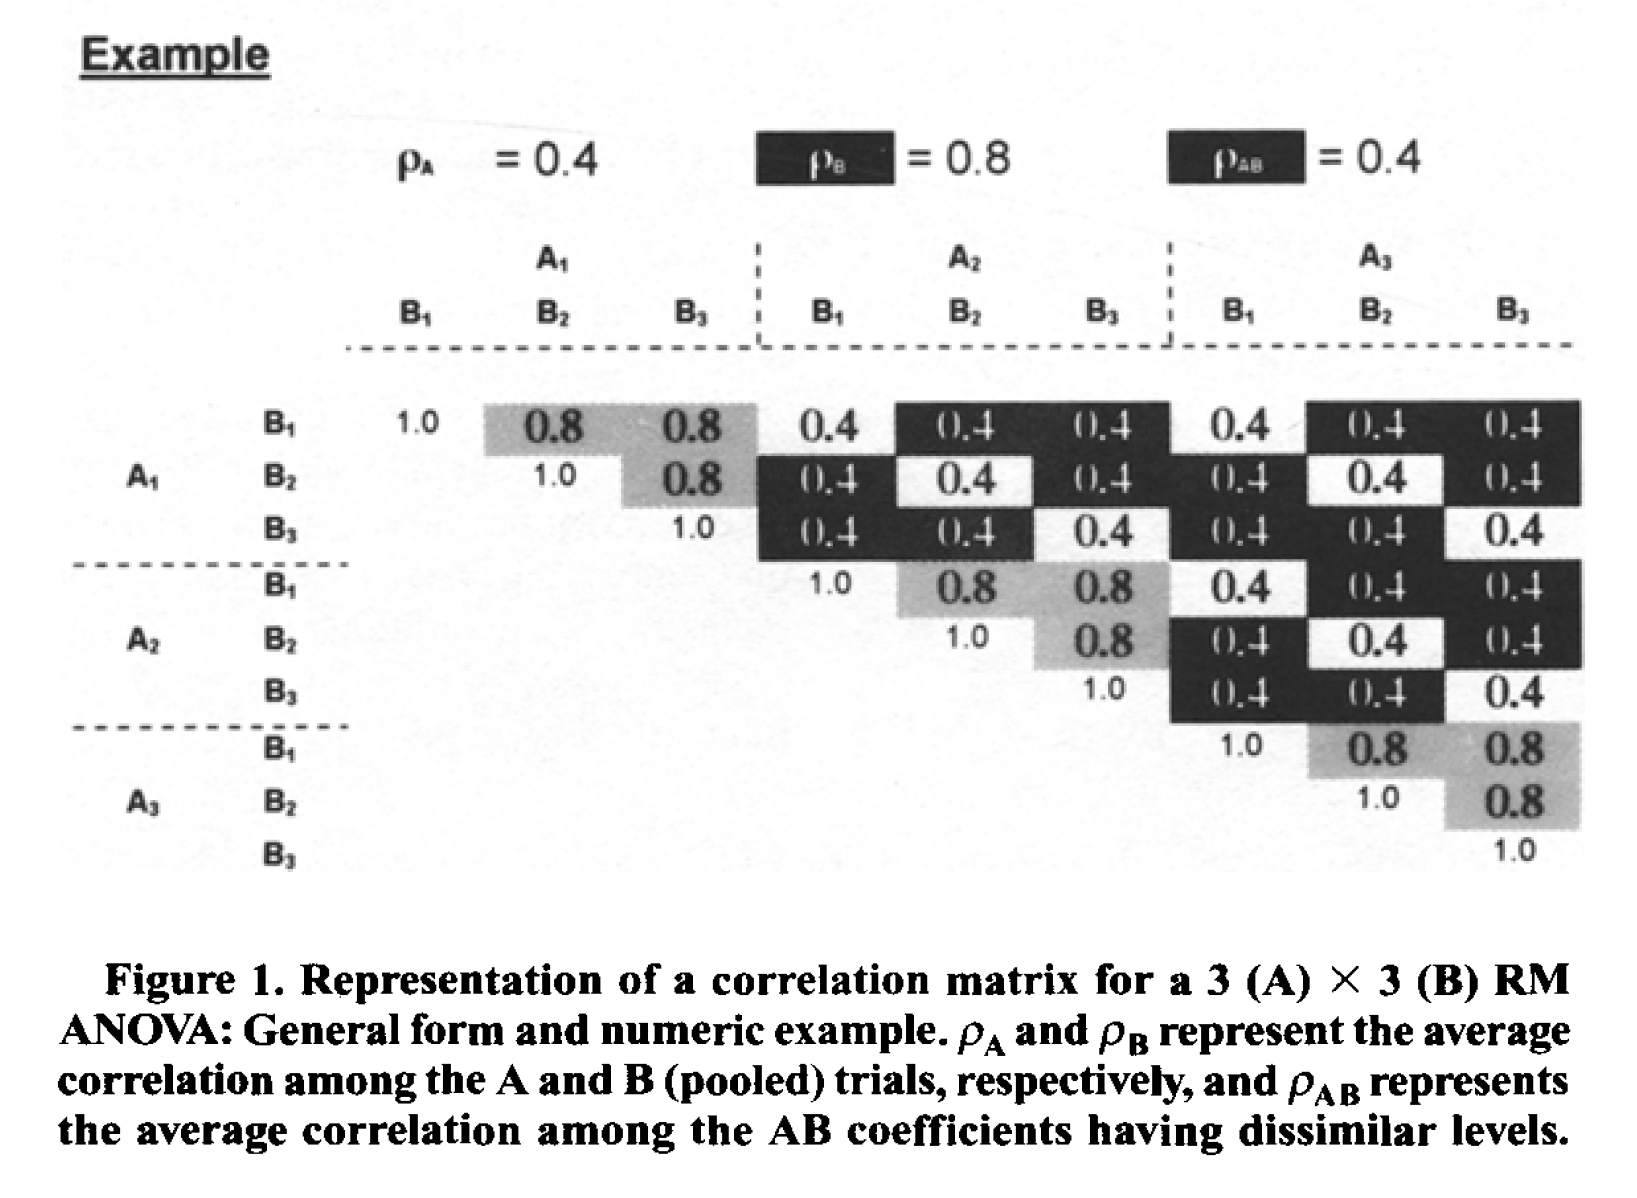
\includegraphics{screenshots/PS2000.png}
\caption{}
\end{figure}

Variances were set to 1 (so all covariance matrices in their simulations
were identical). In this specific example, the white fields are related
to the correlation for the A main effect (these cells have the same
level for B, but different levels of A). The grey cells are related to
the main effect of B (the cells have the same level of A, but different
levels of B). Finally, the black cells are related to the AxB
interaction (they have different levels of A and B). The diagonal (all
1) relate to cells with the same levels of A and B.

Potvin \& Schulz (2000) examine power for 2x2 within ANOVA designs and
develop approximations of the error variance. For a design with 2 within
factors (A and B) these are:

For the main effect of A:
\(\sigma _ { e } ^ { 2 } = \sigma ^ { 2 } ( 1 - \overline { \rho } _ { A } ) + \sigma ^ { 2 } ( q - 1 ) ( \overline { \rho } _ { B } - \overline { \rho } _ { AB } )\)

For the main effectof B:
\(\sigma _ { e } ^ { 2 } = \sigma ^ { 2 } ( 1 - \overline { \rho } _ { B } ) + \sigma ^ { 2 } ( p - 1 ) ( \overline { \rho } _ { A } - \overline { \rho } _ { A B } )\)

For the interaction between A and B:
\(\sigma _ { e } ^ { 2 } = \sigma ^ { 2 } ( 1 - \rho _ { \max } ) - \sigma ^ { 2 } ( \overline { \rho } _ { \min } - \overline { \rho } _ { AB } )\)

We first simulate a within subjects 2x2 ANOVA design.

\begin{Shaded}
\begin{Highlighting}[]
\NormalTok{mu =}\StringTok{ }\KeywordTok{c}\NormalTok{(}\DecValTok{2}\NormalTok{,}\DecValTok{1}\NormalTok{,}\DecValTok{4}\NormalTok{,}\DecValTok{2}\NormalTok{) }
\NormalTok{n <-}\StringTok{ }\DecValTok{20}
\NormalTok{sd <-}\StringTok{ }\DecValTok{5}
\NormalTok{r <-}\StringTok{ }\KeywordTok{c}\NormalTok{(}
  \FloatTok{0.8}\NormalTok{, }\FloatTok{0.5}\NormalTok{, }\FloatTok{0.4}\NormalTok{,}
       \FloatTok{0.4}\NormalTok{, }\FloatTok{0.5}\NormalTok{,}
            \FloatTok{0.8}
\NormalTok{  )}

\NormalTok{string =}\StringTok{ "2w*2w"}
\NormalTok{alpha_level <-}\StringTok{ }\FloatTok{0.05}
\NormalTok{p_adjust =}\StringTok{ "none"}
\NormalTok{labelnames =}\StringTok{ }\KeywordTok{c}\NormalTok{(}\StringTok{"A"}\NormalTok{, }\StringTok{"a1"}\NormalTok{, }\StringTok{"a2"}\NormalTok{, }\StringTok{"B"}\NormalTok{, }\StringTok{"b1"}\NormalTok{, }\StringTok{"b2"}\NormalTok{)}
\NormalTok{design_result <-}\StringTok{ }\KeywordTok{ANOVA_design}\NormalTok{(}\DataTypeTok{string =}\NormalTok{ string,}
                              \DataTypeTok{n =}\NormalTok{ n, }
                              \DataTypeTok{mu =}\NormalTok{ mu, }
                              \DataTypeTok{sd =}\NormalTok{ sd, }
                              \DataTypeTok{r =}\NormalTok{ r, }
                              \DataTypeTok{p_adjust =}\NormalTok{ p_adjust,}
                              \DataTypeTok{labelnames =}\NormalTok{ labelnames)}
\end{Highlighting}
\end{Shaded}

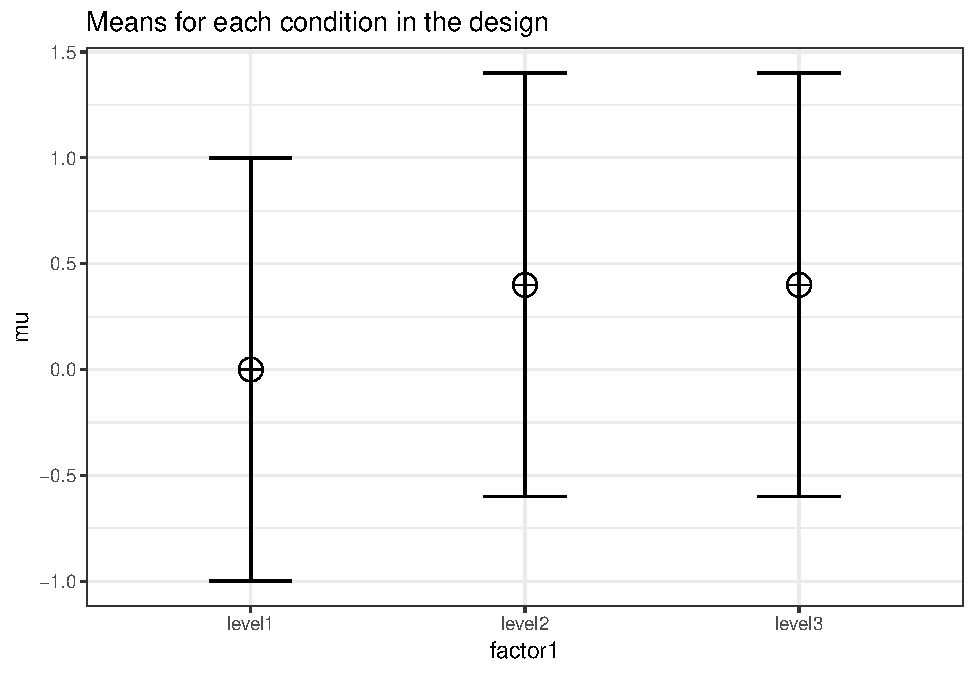
\includegraphics{4.3_analytic_power_functions_files/figure-latex/unnamed-chunk-4-1.pdf}

\begin{Shaded}
\begin{Highlighting}[]
\NormalTok{simulation_result <-}\StringTok{ }\KeywordTok{ANOVA_power}\NormalTok{(design_result, }\DataTypeTok{alpha =} \FloatTok{0.05}\NormalTok{, }\DataTypeTok{nsims =}\NormalTok{ nsims)}
\end{Highlighting}
\end{Shaded}

\begin{verbatim}
## Power and Effect sizes for ANOVA tests
##            power effect size
## anova_A   26.972      0.0984
## anova_B   64.231      0.2448
## anova_A:B 26.866      0.0982
## 
## Power and Effect sizes for contrasts
##                        power effect size
## p_A_a1_B_b1_A_a1_B_b2 27.014     -0.3297
## p_A_a1_B_b1_A_a2_B_b1 39.820      0.4176
## p_A_a1_B_b1_A_a2_B_b2  4.972      0.0003
## p_A_a1_B_b2_A_a2_B_b1 64.220      0.5719
## p_A_a1_B_b2_A_a2_B_b2 13.565      0.2087
## p_A_a2_B_b1_A_a2_B_b2 76.624     -0.6591
\end{verbatim}

Result simulation after 100000 simulations

simulation\_result \textless{}- ANOVA\_power(design\_result, alpha =
0.05, nsims = 100000) Power and Effect sizes for ANOVA tests power
effect size anova\_A 26.849 0.0984 anova\_B 64.091 0.2452 anova\_A:B
26.875 0.0983

Power and Effect sizes for contrasts power effect size
p\_A\_a1\_B\_b1\_A\_a1\_B\_b2 27.052 -0.3298
p\_A\_a1\_B\_b1\_A\_a2\_B\_b1 39.637 0.4162
p\_A\_a1\_B\_b1\_A\_a2\_B\_b2 4.983 -0.0005
p\_A\_a1\_B\_b2\_A\_a2\_B\_b1 64.252 0.5699
p\_A\_a1\_B\_b2\_A\_a2\_B\_b2 13.479 0.2077
p\_A\_a2\_B\_b1\_A\_a2\_B\_b2 76.622 -0.6597

We can try to use the formula in Potvin \& Schutz (2000).

\begin{Shaded}
\begin{Highlighting}[]
\NormalTok{mean_mat <-}\StringTok{ }\KeywordTok{t}\NormalTok{(}\KeywordTok{matrix}\NormalTok{(mu, }
                     \DataTypeTok{nrow =} \DecValTok{2}\NormalTok{,}
                     \DataTypeTok{ncol =} \DecValTok{2}\NormalTok{)) }\CommentTok{#Create a mean matrix}
\KeywordTok{rownames}\NormalTok{(mean_mat) <-}\StringTok{ }\KeywordTok{c}\NormalTok{(}\StringTok{"a1"}\NormalTok{, }\StringTok{"a2"}\NormalTok{)}
\KeywordTok{colnames}\NormalTok{(mean_mat) <-}\StringTok{ }\KeywordTok{c}\NormalTok{(}\StringTok{"b1"}\NormalTok{, }\StringTok{"b2"}\NormalTok{)}
\NormalTok{mean_mat}
\end{Highlighting}
\end{Shaded}

\begin{verbatim}
##    b1 b2
## a1  2  1
## a2  4  2
\end{verbatim}

\begin{Shaded}
\begin{Highlighting}[]
\NormalTok{a1 <-}\StringTok{ }\NormalTok{mean_mat[}\DecValTok{1}\NormalTok{,}\DecValTok{1}\NormalTok{] }\OperatorTok{-}\StringTok{ }\NormalTok{(}\KeywordTok{mean}\NormalTok{(mean_mat) }\OperatorTok{+}\StringTok{ }\NormalTok{(}\KeywordTok{mean}\NormalTok{(mean_mat[}\DecValTok{1}\NormalTok{,]) }\OperatorTok{-}\StringTok{ }\KeywordTok{mean}\NormalTok{(mean_mat)) }\OperatorTok{+}\StringTok{ }\NormalTok{(}\KeywordTok{mean}\NormalTok{(mean_mat[,}\DecValTok{1}\NormalTok{]) }\OperatorTok{-}\StringTok{ }\KeywordTok{mean}\NormalTok{(mean_mat)))}
\NormalTok{a2 <-}\StringTok{ }\NormalTok{mean_mat[}\DecValTok{1}\NormalTok{,}\DecValTok{2}\NormalTok{] }\OperatorTok{-}\StringTok{ }\NormalTok{(}\KeywordTok{mean}\NormalTok{(mean_mat) }\OperatorTok{+}\StringTok{ }\NormalTok{(}\KeywordTok{mean}\NormalTok{(mean_mat[}\DecValTok{1}\NormalTok{,]) }\OperatorTok{-}\StringTok{ }\KeywordTok{mean}\NormalTok{(mean_mat)) }\OperatorTok{+}\StringTok{ }\NormalTok{(}\KeywordTok{mean}\NormalTok{(mean_mat[,}\DecValTok{2}\NormalTok{]) }\OperatorTok{-}\StringTok{ }\KeywordTok{mean}\NormalTok{(mean_mat)))}
\NormalTok{b1 <-}\StringTok{ }\NormalTok{mean_mat[}\DecValTok{2}\NormalTok{,}\DecValTok{1}\NormalTok{] }\OperatorTok{-}\StringTok{ }\NormalTok{(}\KeywordTok{mean}\NormalTok{(mean_mat) }\OperatorTok{+}\StringTok{ }\NormalTok{(}\KeywordTok{mean}\NormalTok{(mean_mat[}\DecValTok{2}\NormalTok{,]) }\OperatorTok{-}\StringTok{ }\KeywordTok{mean}\NormalTok{(mean_mat)) }\OperatorTok{+}\StringTok{ }\NormalTok{(}\KeywordTok{mean}\NormalTok{(mean_mat[,}\DecValTok{1}\NormalTok{]) }\OperatorTok{-}\StringTok{ }\KeywordTok{mean}\NormalTok{(mean_mat)))}
\NormalTok{b2 <-}\StringTok{ }\NormalTok{mean_mat[}\DecValTok{2}\NormalTok{,}\DecValTok{2}\NormalTok{] }\OperatorTok{-}\StringTok{ }\NormalTok{(}\KeywordTok{mean}\NormalTok{(mean_mat) }\OperatorTok{+}\StringTok{ }\NormalTok{(}\KeywordTok{mean}\NormalTok{(mean_mat[}\DecValTok{2}\NormalTok{,]) }\OperatorTok{-}\StringTok{ }\KeywordTok{mean}\NormalTok{(mean_mat)) }\OperatorTok{+}\StringTok{ }\NormalTok{(}\KeywordTok{mean}\NormalTok{(mean_mat[,}\DecValTok{2}\NormalTok{]) }\OperatorTok{-}\StringTok{ }\KeywordTok{mean}\NormalTok{(mean_mat)))}
\KeywordTok{c}\NormalTok{(a1, a2, b1, b2)}
\end{Highlighting}
\end{Shaded}

\begin{verbatim}
## [1] -0.25  0.25  0.25 -0.25
\end{verbatim}

\begin{Shaded}
\begin{Highlighting}[]
\NormalTok{k <-}\StringTok{ }\DecValTok{1} \CommentTok{#one group (because all factors are within)}
\NormalTok{rho_A <-}\StringTok{ }\FloatTok{0.5} \CommentTok{#mean r for factor A}
\NormalTok{rho_B <-}\StringTok{ }\FloatTok{0.8} \CommentTok{#mean r for factor B}
\NormalTok{rho_AB <-}\StringTok{ }\FloatTok{0.4} \CommentTok{#mean r for factor AB}
\NormalTok{alpha <-}\StringTok{ }\FloatTok{0.05}
\NormalTok{sigma <-}\StringTok{ }\NormalTok{sd}

\NormalTok{m_A <-}\StringTok{ }\DecValTok{2} \CommentTok{#levels factor A}
\NormalTok{variance_e_A <-}\StringTok{ }\NormalTok{sigma}\OperatorTok{^}\DecValTok{2} \OperatorTok{*}\StringTok{ }\NormalTok{(}\DecValTok{1} \OperatorTok{-}\StringTok{ }\NormalTok{rho_A) }\OperatorTok{+}\StringTok{ }\NormalTok{sigma}\OperatorTok{^}\DecValTok{2} \OperatorTok{*}\StringTok{ }\NormalTok{(m_A }\OperatorTok{-}\StringTok{ }\DecValTok{1}\NormalTok{) }\OperatorTok{*}\StringTok{ }\NormalTok{(rho_B }\OperatorTok{-}\StringTok{ }\NormalTok{rho_AB) }\CommentTok{#Variance A}
\NormalTok{variance_e_A}
\end{Highlighting}
\end{Shaded}

\begin{verbatim}
## [1] 22.5
\end{verbatim}

\begin{Shaded}
\begin{Highlighting}[]
\NormalTok{m_B <-}\StringTok{ }\DecValTok{2} \CommentTok{#levels factor B}
\NormalTok{variance_e_B <-}\StringTok{ }\NormalTok{sigma}\OperatorTok{^}\DecValTok{2} \OperatorTok{*}\StringTok{ }\NormalTok{(}\DecValTok{1} \OperatorTok{-}\StringTok{ }\NormalTok{rho_B) }\OperatorTok{+}\StringTok{ }\NormalTok{sigma}\OperatorTok{^}\DecValTok{2} \OperatorTok{*}\StringTok{ }\NormalTok{(m_B }\OperatorTok{-}\StringTok{ }\DecValTok{1}\NormalTok{) }\OperatorTok{*}\StringTok{ }\NormalTok{(rho_A }\OperatorTok{-}\StringTok{ }\NormalTok{rho_AB) }\CommentTok{#Variance B}
\NormalTok{variance_e_B}
\end{Highlighting}
\end{Shaded}

\begin{verbatim}
## [1] 7.5
\end{verbatim}

\begin{Shaded}
\begin{Highlighting}[]
\NormalTok{variance_e_AB <-}\StringTok{ }\NormalTok{sigma}\OperatorTok{^}\DecValTok{2} \OperatorTok{*}\StringTok{ }\NormalTok{(}\DecValTok{1} \OperatorTok{-}\StringTok{ }\KeywordTok{max}\NormalTok{(rho_A, rho_B)) }\OperatorTok{-}\StringTok{ }\NormalTok{sigma}\OperatorTok{^}\DecValTok{2} \OperatorTok{*}\StringTok{ }\NormalTok{(}\KeywordTok{min}\NormalTok{(rho_A, rho_B) }\OperatorTok{-}\StringTok{ }\NormalTok{rho_AB) }\CommentTok{#Variance AB}
\NormalTok{variance_e_AB}
\end{Highlighting}
\end{Shaded}

\begin{verbatim}
## [1] 2.5
\end{verbatim}

\begin{Shaded}
\begin{Highlighting}[]
\CommentTok{# Potving & Schutz, 2000, formula 2, p. 348}
\CommentTok{# For main effect A}
\NormalTok{lambda_A <-}\StringTok{ }\NormalTok{n }\OperatorTok{*}\StringTok{ }\NormalTok{m_A }\OperatorTok{*}\StringTok{ }\KeywordTok{sum}\NormalTok{((}\KeywordTok{rowMeans}\NormalTok{(mean_mat)}\OperatorTok{-}\KeywordTok{mean}\NormalTok{(}\KeywordTok{rowMeans}\NormalTok{(mean_mat)))}\OperatorTok{^}\DecValTok{2}\NormalTok{)}\OperatorTok{/}\NormalTok{variance_e_A }
\NormalTok{lambda_A}
\end{Highlighting}
\end{Shaded}

\begin{verbatim}
## [1] 2
\end{verbatim}

\begin{Shaded}
\begin{Highlighting}[]
\NormalTok{df1 <-}\StringTok{ }\NormalTok{(m_A }\OperatorTok{-}\StringTok{ }\DecValTok{1}\NormalTok{) }\CommentTok{#calculate degrees of freedom 1 - ignoring the * e sphericity correction}
\NormalTok{df2 <-}\StringTok{ }\NormalTok{(n }\OperatorTok{-}\StringTok{ }\NormalTok{k) }\OperatorTok{*}\StringTok{ }\NormalTok{(m_A }\OperatorTok{-}\StringTok{ }\DecValTok{1}\NormalTok{) }\CommentTok{#calculate degrees of freedom 2}
\NormalTok{F_critical <-}\StringTok{ }\KeywordTok{qf}\NormalTok{(alpha, }\CommentTok{# critical F-vaue}
\NormalTok{                 df1,}
\NormalTok{                 df2, }
                 \DataTypeTok{lower.tail=}\OtherTok{FALSE}\NormalTok{) }

\NormalTok{pow_A <-}\StringTok{ }\KeywordTok{pf}\NormalTok{(}\KeywordTok{qf}\NormalTok{(alpha, }\CommentTok{#power }
\NormalTok{             df1, }
\NormalTok{             df2, }
             \DataTypeTok{lower.tail =} \OtherTok{FALSE}\NormalTok{), }
\NormalTok{          df1, }
\NormalTok{          df2, }
\NormalTok{          lambda_A, }
          \DataTypeTok{lower.tail =} \OtherTok{FALSE}\NormalTok{)}

\NormalTok{lambda_B <-}\StringTok{ }\NormalTok{n }\OperatorTok{*}\StringTok{ }\NormalTok{m_B }\OperatorTok{*}\StringTok{ }\KeywordTok{sum}\NormalTok{((}\KeywordTok{colMeans}\NormalTok{(mean_mat)}\OperatorTok{-}\KeywordTok{mean}\NormalTok{(}\KeywordTok{colMeans}\NormalTok{(mean_mat)))}\OperatorTok{^}\DecValTok{2}\NormalTok{)}\OperatorTok{/}\NormalTok{variance_e_B }
\NormalTok{lambda_B}
\end{Highlighting}
\end{Shaded}

\begin{verbatim}
## [1] 6
\end{verbatim}

\begin{Shaded}
\begin{Highlighting}[]
\NormalTok{df1 <-}\StringTok{ }\NormalTok{(m_B }\OperatorTok{-}\StringTok{ }\DecValTok{1}\NormalTok{) }\CommentTok{#calculate degrees of freedom 1}
\NormalTok{df2 <-}\StringTok{ }\NormalTok{(n }\OperatorTok{-}\StringTok{ }\NormalTok{k) }\OperatorTok{*}\StringTok{ }\NormalTok{(m_B }\OperatorTok{-}\StringTok{ }\DecValTok{1}\NormalTok{) }\CommentTok{#calculate degrees of freedom 2}
\NormalTok{F_critical <-}\StringTok{ }\KeywordTok{qf}\NormalTok{(alpha, }\CommentTok{# critical F-vaue}
\NormalTok{                 df1,}
\NormalTok{                 df2, }
                 \DataTypeTok{lower.tail=}\OtherTok{FALSE}\NormalTok{) }

\NormalTok{pow_B <-}\StringTok{ }\KeywordTok{pf}\NormalTok{(}\KeywordTok{qf}\NormalTok{(alpha, }\CommentTok{#power }
\NormalTok{             df1, }
\NormalTok{             df2, }
             \DataTypeTok{lower.tail =} \OtherTok{FALSE}\NormalTok{), }
\NormalTok{          df1, }
\NormalTok{          df2, }
\NormalTok{          lambda_B, }
          \DataTypeTok{lower.tail =} \OtherTok{FALSE}\NormalTok{)}

\NormalTok{lambda_AB <-}\StringTok{ }\NormalTok{n }\OperatorTok{*}\StringTok{ }\KeywordTok{sqrt}\NormalTok{(}\KeywordTok{sum}\NormalTok{(}\KeywordTok{c}\NormalTok{(a1, a2, b1, b2)}\OperatorTok{^}\DecValTok{2}\NormalTok{)}\OperatorTok{/}\KeywordTok{length}\NormalTok{(mu))}\OperatorTok{/}\StringTok{ }\NormalTok{variance_e_AB }
\NormalTok{lambda_AB}
\end{Highlighting}
\end{Shaded}

\begin{verbatim}
## [1] 2
\end{verbatim}

\begin{Shaded}
\begin{Highlighting}[]
\NormalTok{df1 <-}\StringTok{ }\NormalTok{(m_A }\OperatorTok{-}\StringTok{ }\DecValTok{1}\NormalTok{)}\OperatorTok{*}\NormalTok{(m_B }\OperatorTok{-}\StringTok{ }\DecValTok{1}\NormalTok{)  }\CommentTok{#calculate degrees of freedom 1}
\NormalTok{df2 <-}\StringTok{ }\NormalTok{(n }\OperatorTok{-}\StringTok{ }\NormalTok{k) }\OperatorTok{*}\StringTok{ }\NormalTok{(m_A }\OperatorTok{-}\StringTok{ }\DecValTok{1}\NormalTok{) }\OperatorTok{*}\StringTok{ }\NormalTok{(m_B }\OperatorTok{-}\StringTok{ }\DecValTok{1}\NormalTok{) }\CommentTok{#calculate degrees of freedom 2}
\NormalTok{F_critical <-}\StringTok{ }\KeywordTok{qf}\NormalTok{(alpha, }\CommentTok{# critical F-vaue}
\NormalTok{                 df1,}
\NormalTok{                 df2, }
                 \DataTypeTok{lower.tail=}\OtherTok{FALSE}\NormalTok{) }

\NormalTok{pow_AB <-}\StringTok{ }\KeywordTok{pf}\NormalTok{(}\KeywordTok{qf}\NormalTok{(alpha, }\CommentTok{#power }
\NormalTok{             df1, }
\NormalTok{             df2, }
             \DataTypeTok{lower.tail =} \OtherTok{FALSE}\NormalTok{), }
\NormalTok{          df1, }
\NormalTok{          df2, }
\NormalTok{          lambda_AB, }
          \DataTypeTok{lower.tail =} \OtherTok{FALSE}\NormalTok{)}
\NormalTok{pow_A}
\end{Highlighting}
\end{Shaded}

\begin{verbatim}
## [1] 0.2691752
\end{verbatim}

\begin{Shaded}
\begin{Highlighting}[]
\NormalTok{pow_B}
\end{Highlighting}
\end{Shaded}

\begin{verbatim}
## [1] 0.6422587
\end{verbatim}

\begin{Shaded}
\begin{Highlighting}[]
\NormalTok{pow_AB}
\end{Highlighting}
\end{Shaded}

\begin{verbatim}
## [1] 0.2691752
\end{verbatim}

We see the 26.9 and 64.2, and 26.9 correspond to the results of the
simulation quite closely.

\section{Variation 2x2 within design}\label{variation-2x2-within-design}

We first simulate a within subjects 2x2 ANOVA design.

\begin{Shaded}
\begin{Highlighting}[]
\NormalTok{mu =}\StringTok{ }\KeywordTok{c}\NormalTok{(}\DecValTok{3}\NormalTok{,}\DecValTok{1}\NormalTok{,}\DecValTok{4}\NormalTok{,}\DecValTok{2}\NormalTok{) }
\NormalTok{n <-}\StringTok{ }\DecValTok{20}
\NormalTok{sd <-}\StringTok{ }\DecValTok{5}
\NormalTok{r <-}\StringTok{ }\KeywordTok{c}\NormalTok{(}
  \FloatTok{0.8}\NormalTok{, }\FloatTok{0.5}\NormalTok{, }\FloatTok{0.5}\NormalTok{,}
       \FloatTok{0.5}\NormalTok{, }\FloatTok{0.5}\NormalTok{,}
            \FloatTok{0.8}
\NormalTok{  )}

\NormalTok{string =}\StringTok{ "2w*2w"}
\NormalTok{alpha_level <-}\StringTok{ }\FloatTok{0.05}
\NormalTok{p_adjust =}\StringTok{ "none"}
\NormalTok{labelnames =}\StringTok{ }\KeywordTok{c}\NormalTok{(}\StringTok{"A"}\NormalTok{, }\StringTok{"a1"}\NormalTok{, }\StringTok{"a2"}\NormalTok{, }\StringTok{"B"}\NormalTok{, }\StringTok{"b1"}\NormalTok{, }\StringTok{"b2"}\NormalTok{)}
\NormalTok{design_result <-}\StringTok{ }\KeywordTok{ANOVA_design}\NormalTok{(}\DataTypeTok{string =}\NormalTok{ string,}
                              \DataTypeTok{n =}\NormalTok{ n, }
                              \DataTypeTok{mu =}\NormalTok{ mu, }
                              \DataTypeTok{sd =}\NormalTok{ sd, }
                              \DataTypeTok{r =}\NormalTok{ r, }
                              \DataTypeTok{p_adjust =}\NormalTok{ p_adjust,}
                              \DataTypeTok{labelnames =}\NormalTok{ labelnames)}
\end{Highlighting}
\end{Shaded}

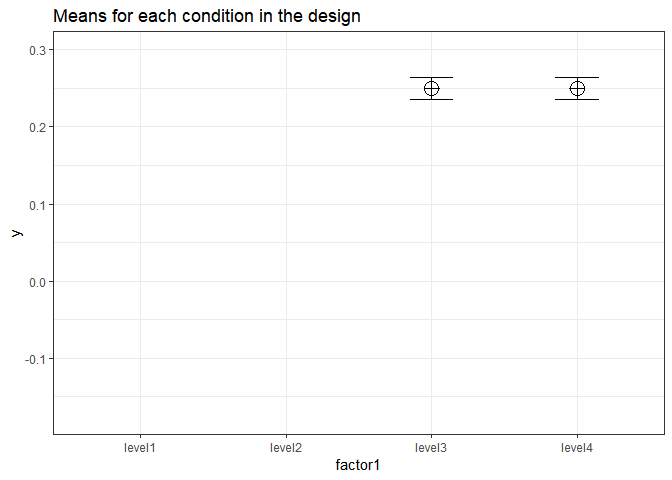
\includegraphics{4.3_analytic_power_functions_files/figure-latex/unnamed-chunk-6-1.pdf}

\begin{Shaded}
\begin{Highlighting}[]
\NormalTok{simulation_result <-}\StringTok{ }\KeywordTok{ANOVA_power}\NormalTok{(design_result, }\DataTypeTok{alpha =} \FloatTok{0.05}\NormalTok{, }\DataTypeTok{nsims =}\NormalTok{ nsims)}
\end{Highlighting}
\end{Shaded}

\begin{verbatim}
## Power and Effect sizes for ANOVA tests
##            power effect size
## anova_A   15.815      0.0567
## anova_B   96.657      0.4641
## anova_A:B  5.068      0.0241
## 
## Power and Effect sizes for contrasts
##                        power effect size
## p_A_a1_B_b1_A_a1_B_b2 76.372     -0.6580
## p_A_a1_B_b1_A_a2_B_b1 13.489      0.2086
## p_A_a1_B_b1_A_a2_B_b2 13.626     -0.2082
## p_A_a1_B_b2_A_a2_B_b1 71.970      0.6252
## p_A_a1_B_b2_A_a2_B_b2 13.606      0.2084
## p_A_a2_B_b1_A_a2_B_b2 76.770     -0.6592
\end{verbatim}

Now the analytic solution.

\begin{Shaded}
\begin{Highlighting}[]
\NormalTok{mean_mat <-}\StringTok{ }\KeywordTok{t}\NormalTok{(}\KeywordTok{matrix}\NormalTok{(mu, }
                     \DataTypeTok{nrow =} \DecValTok{2}\NormalTok{,}
                     \DataTypeTok{ncol =} \DecValTok{2}\NormalTok{)) }\CommentTok{#Create a mean matrix}
\KeywordTok{rownames}\NormalTok{(mean_mat) <-}\StringTok{ }\KeywordTok{c}\NormalTok{(}\StringTok{"a1"}\NormalTok{, }\StringTok{"a2"}\NormalTok{)}
\KeywordTok{colnames}\NormalTok{(mean_mat) <-}\StringTok{ }\KeywordTok{c}\NormalTok{(}\StringTok{"b1"}\NormalTok{, }\StringTok{"b2"}\NormalTok{)}
\NormalTok{mean_mat}
\end{Highlighting}
\end{Shaded}

\begin{verbatim}
##    b1 b2
## a1  3  1
## a2  4  2
\end{verbatim}

\begin{Shaded}
\begin{Highlighting}[]
\NormalTok{a1 <-}\StringTok{ }\NormalTok{mean_mat[}\DecValTok{1}\NormalTok{,}\DecValTok{1}\NormalTok{] }\OperatorTok{-}\StringTok{ }\NormalTok{(}\KeywordTok{mean}\NormalTok{(mean_mat) }\OperatorTok{+}\StringTok{ }\NormalTok{(}\KeywordTok{mean}\NormalTok{(mean_mat[}\DecValTok{1}\NormalTok{,]) }\OperatorTok{-}\StringTok{ }\KeywordTok{mean}\NormalTok{(mean_mat)) }\OperatorTok{+}\StringTok{ }\NormalTok{(}\KeywordTok{mean}\NormalTok{(mean_mat[,}\DecValTok{1}\NormalTok{]) }\OperatorTok{-}\StringTok{ }\KeywordTok{mean}\NormalTok{(mean_mat)))}
\NormalTok{a2 <-}\StringTok{ }\NormalTok{mean_mat[}\DecValTok{1}\NormalTok{,}\DecValTok{2}\NormalTok{] }\OperatorTok{-}\StringTok{ }\NormalTok{(}\KeywordTok{mean}\NormalTok{(mean_mat) }\OperatorTok{+}\StringTok{ }\NormalTok{(}\KeywordTok{mean}\NormalTok{(mean_mat[}\DecValTok{1}\NormalTok{,]) }\OperatorTok{-}\StringTok{ }\KeywordTok{mean}\NormalTok{(mean_mat)) }\OperatorTok{+}\StringTok{ }\NormalTok{(}\KeywordTok{mean}\NormalTok{(mean_mat[,}\DecValTok{2}\NormalTok{]) }\OperatorTok{-}\StringTok{ }\KeywordTok{mean}\NormalTok{(mean_mat)))}
\NormalTok{b1 <-}\StringTok{ }\NormalTok{mean_mat[}\DecValTok{2}\NormalTok{,}\DecValTok{1}\NormalTok{] }\OperatorTok{-}\StringTok{ }\NormalTok{(}\KeywordTok{mean}\NormalTok{(mean_mat) }\OperatorTok{+}\StringTok{ }\NormalTok{(}\KeywordTok{mean}\NormalTok{(mean_mat[}\DecValTok{2}\NormalTok{,]) }\OperatorTok{-}\StringTok{ }\KeywordTok{mean}\NormalTok{(mean_mat)) }\OperatorTok{+}\StringTok{ }\NormalTok{(}\KeywordTok{mean}\NormalTok{(mean_mat[,}\DecValTok{1}\NormalTok{]) }\OperatorTok{-}\StringTok{ }\KeywordTok{mean}\NormalTok{(mean_mat)))}
\NormalTok{b2 <-}\StringTok{ }\NormalTok{mean_mat[}\DecValTok{2}\NormalTok{,}\DecValTok{2}\NormalTok{] }\OperatorTok{-}\StringTok{ }\NormalTok{(}\KeywordTok{mean}\NormalTok{(mean_mat) }\OperatorTok{+}\StringTok{ }\NormalTok{(}\KeywordTok{mean}\NormalTok{(mean_mat[}\DecValTok{2}\NormalTok{,]) }\OperatorTok{-}\StringTok{ }\KeywordTok{mean}\NormalTok{(mean_mat)) }\OperatorTok{+}\StringTok{ }\NormalTok{(}\KeywordTok{mean}\NormalTok{(mean_mat[,}\DecValTok{2}\NormalTok{]) }\OperatorTok{-}\StringTok{ }\KeywordTok{mean}\NormalTok{(mean_mat)))}
\KeywordTok{c}\NormalTok{(a1, a2, b1, b2)}
\end{Highlighting}
\end{Shaded}

\begin{verbatim}
## [1] 0 0 0 0
\end{verbatim}

\begin{Shaded}
\begin{Highlighting}[]
\NormalTok{k <-}\StringTok{ }\DecValTok{1} \CommentTok{#one group (because all factors are within)}
\NormalTok{rho_A <-}\StringTok{ }\FloatTok{0.5} \CommentTok{#mean r for factor A}
\NormalTok{rho_B <-}\StringTok{ }\FloatTok{0.8} \CommentTok{#mean r for factor B}
\NormalTok{rho_AB <-}\StringTok{ }\FloatTok{0.4} \CommentTok{#mean r for factor AB}
\NormalTok{alpha <-}\StringTok{ }\FloatTok{0.05}
\NormalTok{sigma <-}\StringTok{ }\NormalTok{sd}

\NormalTok{m_A <-}\StringTok{ }\DecValTok{2} \CommentTok{#levels factor A}
\NormalTok{variance_e_A <-}\StringTok{ }\NormalTok{sigma}\OperatorTok{^}\DecValTok{2} \OperatorTok{*}\StringTok{ }\NormalTok{(}\DecValTok{1} \OperatorTok{-}\StringTok{ }\NormalTok{rho_A) }\OperatorTok{+}\StringTok{ }\NormalTok{sigma}\OperatorTok{^}\DecValTok{2} \OperatorTok{*}\StringTok{ }\NormalTok{(m_A }\OperatorTok{-}\StringTok{ }\DecValTok{1}\NormalTok{) }\OperatorTok{*}\StringTok{ }\NormalTok{(rho_B }\OperatorTok{-}\StringTok{ }\NormalTok{rho_AB) }\CommentTok{#Variance A}
\NormalTok{variance_e_A}
\end{Highlighting}
\end{Shaded}

\begin{verbatim}
## [1] 22.5
\end{verbatim}

\begin{Shaded}
\begin{Highlighting}[]
\NormalTok{m_B <-}\StringTok{ }\DecValTok{2} \CommentTok{#levels factor B}
\NormalTok{variance_e_B <-}\StringTok{ }\NormalTok{sigma}\OperatorTok{^}\DecValTok{2} \OperatorTok{*}\StringTok{ }\NormalTok{(}\DecValTok{1} \OperatorTok{-}\StringTok{ }\NormalTok{rho_B) }\OperatorTok{+}\StringTok{ }\NormalTok{sigma}\OperatorTok{^}\DecValTok{2} \OperatorTok{*}\StringTok{ }\NormalTok{(m_B }\OperatorTok{-}\StringTok{ }\DecValTok{1}\NormalTok{) }\OperatorTok{*}\StringTok{ }\NormalTok{(rho_A }\OperatorTok{-}\StringTok{ }\NormalTok{rho_AB) }\CommentTok{#Variance B}
\NormalTok{variance_e_B}
\end{Highlighting}
\end{Shaded}

\begin{verbatim}
## [1] 7.5
\end{verbatim}

\begin{Shaded}
\begin{Highlighting}[]
\NormalTok{variance_e_AB <-}\StringTok{ }\NormalTok{sigma}\OperatorTok{^}\DecValTok{2} \OperatorTok{*}\StringTok{ }\NormalTok{(}\DecValTok{1} \OperatorTok{-}\StringTok{ }\KeywordTok{max}\NormalTok{(rho_A, rho_B)) }\OperatorTok{-}\StringTok{ }\NormalTok{sigma}\OperatorTok{^}\DecValTok{2} \OperatorTok{*}\StringTok{ }\NormalTok{(}\KeywordTok{min}\NormalTok{(rho_A, rho_B) }\OperatorTok{-}\StringTok{ }\NormalTok{rho_AB) }\CommentTok{#Variance AB}
\NormalTok{variance_e_AB}
\end{Highlighting}
\end{Shaded}

\begin{verbatim}
## [1] 2.5
\end{verbatim}

\begin{Shaded}
\begin{Highlighting}[]
\CommentTok{# Potving & Schutz, 2000, formula 2, p. 348}
\CommentTok{# For main effect A}
\NormalTok{lambda_A <-}\StringTok{ }\NormalTok{n }\OperatorTok{*}\StringTok{ }\NormalTok{m_A }\OperatorTok{*}\StringTok{ }\KeywordTok{sum}\NormalTok{((}\KeywordTok{rowMeans}\NormalTok{(mean_mat)}\OperatorTok{-}\KeywordTok{mean}\NormalTok{(}\KeywordTok{rowMeans}\NormalTok{(mean_mat)))}\OperatorTok{^}\DecValTok{2}\NormalTok{)}\OperatorTok{/}\NormalTok{variance_e_A }
\NormalTok{lambda_A}
\end{Highlighting}
\end{Shaded}

\begin{verbatim}
## [1] 0.8888889
\end{verbatim}

\begin{Shaded}
\begin{Highlighting}[]
\NormalTok{df1 <-}\StringTok{ }\NormalTok{(m_A }\OperatorTok{-}\StringTok{ }\DecValTok{1}\NormalTok{) }\CommentTok{#calculate degrees of freedom 1 - ignoring the * e sphericity correction}
\NormalTok{df2 <-}\StringTok{ }\NormalTok{(n }\OperatorTok{-}\StringTok{ }\NormalTok{k) }\OperatorTok{*}\StringTok{ }\NormalTok{(m_A }\OperatorTok{-}\StringTok{ }\DecValTok{1}\NormalTok{) }\CommentTok{#calculate degrees of freedom 2}
\NormalTok{F_critical <-}\StringTok{ }\KeywordTok{qf}\NormalTok{(alpha, }\CommentTok{# critical F-vaue}
\NormalTok{                 df1,}
\NormalTok{                 df2, }
                 \DataTypeTok{lower.tail=}\OtherTok{FALSE}\NormalTok{) }

\NormalTok{pow_A <-}\StringTok{ }\KeywordTok{pf}\NormalTok{(}\KeywordTok{qf}\NormalTok{(alpha, }\CommentTok{#power }
\NormalTok{             df1, }
\NormalTok{             df2, }
             \DataTypeTok{lower.tail =} \OtherTok{FALSE}\NormalTok{), }
\NormalTok{          df1, }
\NormalTok{          df2, }
\NormalTok{          lambda_A, }
          \DataTypeTok{lower.tail =} \OtherTok{FALSE}\NormalTok{)}

\NormalTok{lambda_B <-}\StringTok{ }\NormalTok{n }\OperatorTok{*}\StringTok{ }\NormalTok{m_B }\OperatorTok{*}\StringTok{ }\KeywordTok{sum}\NormalTok{((}\KeywordTok{colMeans}\NormalTok{(mean_mat)}\OperatorTok{-}\KeywordTok{mean}\NormalTok{(}\KeywordTok{colMeans}\NormalTok{(mean_mat)))}\OperatorTok{^}\DecValTok{2}\NormalTok{)}\OperatorTok{/}\NormalTok{variance_e_B }
\NormalTok{lambda_B}
\end{Highlighting}
\end{Shaded}

\begin{verbatim}
## [1] 10.66667
\end{verbatim}

\begin{Shaded}
\begin{Highlighting}[]
\NormalTok{df1 <-}\StringTok{ }\NormalTok{(m_B }\OperatorTok{-}\StringTok{ }\DecValTok{1}\NormalTok{) }\CommentTok{#calculate degrees of freedom 1}
\NormalTok{df2 <-}\StringTok{ }\NormalTok{(n }\OperatorTok{-}\StringTok{ }\NormalTok{k) }\OperatorTok{*}\StringTok{ }\NormalTok{(m_B }\OperatorTok{-}\StringTok{ }\DecValTok{1}\NormalTok{) }\CommentTok{#calculate degrees of freedom 2}
\NormalTok{F_critical <-}\StringTok{ }\KeywordTok{qf}\NormalTok{(alpha, }\CommentTok{# critical F-vaue}
\NormalTok{                 df1,}
\NormalTok{                 df2, }
                 \DataTypeTok{lower.tail=}\OtherTok{FALSE}\NormalTok{) }

\NormalTok{pow_B <-}\StringTok{ }\KeywordTok{pf}\NormalTok{(}\KeywordTok{qf}\NormalTok{(alpha, }\CommentTok{#power }
\NormalTok{             df1, }
\NormalTok{             df2, }
             \DataTypeTok{lower.tail =} \OtherTok{FALSE}\NormalTok{), }
\NormalTok{          df1, }
\NormalTok{          df2, }
\NormalTok{          lambda_B, }
          \DataTypeTok{lower.tail =} \OtherTok{FALSE}\NormalTok{)}

\NormalTok{lambda_AB <-}\StringTok{ }\NormalTok{n }\OperatorTok{*}\StringTok{ }\KeywordTok{sqrt}\NormalTok{(}\KeywordTok{sum}\NormalTok{(}\KeywordTok{c}\NormalTok{(a1, a2, b1, b2)}\OperatorTok{^}\DecValTok{2}\NormalTok{)}\OperatorTok{/}\KeywordTok{length}\NormalTok{(mu))}\OperatorTok{/}\StringTok{ }\NormalTok{variance_e_AB }
\NormalTok{lambda_AB}
\end{Highlighting}
\end{Shaded}

\begin{verbatim}
## [1] 0
\end{verbatim}

\begin{Shaded}
\begin{Highlighting}[]
\NormalTok{df1 <-}\StringTok{ }\NormalTok{(m_A }\OperatorTok{-}\StringTok{ }\DecValTok{1}\NormalTok{)}\OperatorTok{*}\NormalTok{(m_B }\OperatorTok{-}\StringTok{ }\DecValTok{1}\NormalTok{)  }\CommentTok{#calculate degrees of freedom 1}
\NormalTok{df2 <-}\StringTok{ }\NormalTok{(n }\OperatorTok{-}\StringTok{ }\NormalTok{k) }\OperatorTok{*}\StringTok{ }\NormalTok{(m_A }\OperatorTok{-}\StringTok{ }\DecValTok{1}\NormalTok{) }\OperatorTok{*}\StringTok{ }\NormalTok{(m_B }\OperatorTok{-}\StringTok{ }\DecValTok{1}\NormalTok{) }\CommentTok{#calculate degrees of freedom 2}
\NormalTok{F_critical <-}\StringTok{ }\KeywordTok{qf}\NormalTok{(alpha, }\CommentTok{# critical F-vaue}
\NormalTok{                 df1,}
\NormalTok{                 df2, }
                 \DataTypeTok{lower.tail=}\OtherTok{FALSE}\NormalTok{) }

\NormalTok{pow_AB <-}\StringTok{ }\KeywordTok{pf}\NormalTok{(}\KeywordTok{qf}\NormalTok{(alpha, }\CommentTok{#power }
\NormalTok{             df1, }
\NormalTok{             df2, }
             \DataTypeTok{lower.tail =} \OtherTok{FALSE}\NormalTok{), }
\NormalTok{          df1, }
\NormalTok{          df2, }
\NormalTok{          lambda_AB, }
          \DataTypeTok{lower.tail =} \OtherTok{FALSE}\NormalTok{)}
\NormalTok{pow_A}
\end{Highlighting}
\end{Shaded}

\begin{verbatim}
## [1] 0.1457747
\end{verbatim}

\begin{Shaded}
\begin{Highlighting}[]
\NormalTok{pow_B}
\end{Highlighting}
\end{Shaded}

\begin{verbatim}
## [1] 0.8722533
\end{verbatim}

\begin{Shaded}
\begin{Highlighting}[]
\NormalTok{pow_AB}
\end{Highlighting}
\end{Shaded}

\begin{verbatim}
## [1] 0.05
\end{verbatim}


\end{document}
